% SOURCE docs/release/2026-10-29/source/docs/writing-repair/2026-10-29/src/66540a8f29f1b949.tex CHAR 0
\chapter{Choosing the capabilities worth assembling}
\label{scisyn:software}

A bank does not buy an average treatment effect. It buys a better decision:
which customers to contact, which price to quote, which branches to reorganise,
or which experiment to fund. Software is useful when its answer bears on that
decision and its assumptions are credible in the setting. A method that answers
a narrower question accurately can be more valuable than an ambitious system
whose output is difficult to interpret.

The detailed comparisons in this monograph support selective reuse. The first
proposal should assemble a small number of named statistical procedures around
a common description of the decision. It should retain a second implementation
where disagreement could expose a consequential mistake. It should not promise
to reproduce every package in one language. The development expense of such a
rewrite is certain; the benefit remains to be demonstrated.

The comparison below draws on the retained technical sources and their dated
versions. It is a synthesis of those inspections, not a new census of current
releases. Research coverage ends on 7 October 2026; acquisition after that date
does not establish historical availability of a mutable manual. A documented
procedure, an executed example and a proposed integration are different kinds
of evidence. Commercial tools are compared by their documented procedures;
unobserved functions remain unknown rather than being treated as absent.

\section{Discovering relationships and identifying effects}

\subsection{1. Discovery from independent observations}
For a cross-sectional customer study, the first choice is the set of assumptions
under which conditional independence or a score can reveal useful structure.
The inspected R pcalg, Python causal-learn and Java Tetrad implementations provide
concrete comparison routes for PC. They expose choices about independence tests,
search and orientation. Using the same algorithm name does not align those
choices. A graph with unresolved directions is a legitimate result, not an
unfinished diagram to be completed by managerial intuition.
\citep{exec13_pcalg_reuse_primary,v12_sw_causallearn,exec13_java_tetrad}

A restricted PC comparison needs one primary implementation and another
whose choices can be inspected independently. The independence test, sampling
unit, significance level and treatment of orientation conflicts determine
whether their outputs can be compared.
Porting the search into a new language is not justified by the proposal's
present evidence. Score-based, functional and continuous-optimisation methods
belong beside PC as different modelling choices, rather than votes for a
majority graph. In particular, agreement among bridges to the same underlying
engine is not independent corroboration. The software recommendation changes
if the bank needs a mixed-data model, hidden common causes or repeated records:
those needs require a separate statistical comparison before an interface is
chosen.

\subsection{2. Hidden common causes, selection and equivalent graphs}
An apparent connection between contact and repayment may arise because staff
recognise distress that the database does not record. Under such circumstances
an analysis assuming no hidden common causes can be precise about the wrong
model. The inspected discovery sources distinguish procedures such as PC and
FCI and different graph representations. An algorithmic orientation conflict
must not be reinterpreted as an established hidden common cause merely because
the display uses a similar pair of arrowheads.
\citep{v12_sw_causallearn,exec13_pcalg_reuse_primary}

The partially directed or ancestral graph determines a range of intervention
conclusions under its stated assumptions. A latent-variable route also needs
an explicit interpretation of its endpoints. Selecting one convenient
orientation would instead report an unidentified effect as identified. This is a rejection of an inference, not of a software
family. Where observationally equivalent models imply different lending
decisions, additional timing knowledge or experimental information is the
valuable purchase. Another graph visualiser cannot supply that information.

\subsection{3. Time, interventions and changing regimes}
Repeated customer observations contain both persistence and common shocks.
The retained Tigramite sources distinguish discovery methods, tests, lag
conventions, graph classes and effect calculations conditional on a supplied
graph. Their observation and masking rules matter when a calendar period is
missing. A row after a missing month is not necessarily the next economic
period. Commercial dynamic-network and structural time-series routes are
useful alternatives, but a supplied temporal model and a discovered model
answer different questions.
\citep{exec23_tigramite_reuse_source,exec13_ct_genie_dbn,exec13_ct_stata_svar}

Temporal integration therefore depends on the original calendar, observation
availability and the allowed intervention. Evidence from multiple regimes
has a different interpretation from an assumption that one stationary regime
describes all years. A rate change during a funding crisis need not have the response seen
in ordinary months. A lagged prediction improvement alone does not identify a general temporal
effect. The first comparison should assess whether plausible
lag and regime choices change the decision, with graph ambiguity carried into
the effect calculation.

\subsection{4. Adjustment, identification and counterfactual questions}
The bank must distinguish identification of an intervention distribution from
evaluation of a structural model that somebody has supplied. Ananke's inspected
identification and model-oracle interfaces make this distinction concrete.
aGrUM and pyAgrum likewise combine graphical, symbolic and numerical facilities
whose individual meanings must be preserved. A symbolic expression may still
require conditional distributions unsupported by the observed population.
\citep{exec24_ananke_source,exec19_cxx_identification_source,exec24_agrum_source}

Symbolic identification determines what can be learned before an estimator
is selected. Model-based counterfactual simulation answers a separate question
conditional on the supplied structure. A simulation from that structure
therefore cannot establish identification from observational records.
An R, Python or C++ route is acceptable only if it preserves the query,
conditioning set, hidden-variable assumptions and support requirements. The
unresolved commercial comparison concerns exact query semantics and supported
model classes; a capability label such as causal analysis is insufficient.

\section{Estimating benefits from actions and repeated policies}

\subsection{5. Average and heterogeneous effects}
EconML's residual-regression formulation illustrates why the final effect model
matters as much as the prediction methods used to remove confounding. In a
binary-treatment setting with sufficient observed adjustment information $S$,
write $e(S)=P(A=1\mid S)$ and $\tau(S)=E[Y(1)-Y(0)\mid S]$. With exact nuisance
functions and a constant final coefficient, the population projection is
\[
 \theta_* = \frac{E[e(S)\{1-e(S)\}\tau(S)]}
                   {E[e(S)\{1-e(S)\}]}.
\]
The average benefit for the target population is instead $E[\tau(S)]$.
These coincide under a constant effect, but need not do so otherwise. This
derivation concerns a restricted specification, not every EconML estimator.
\citep{exec19_econml_source}

An explicit specification separates adjustment variables, effect modifiers
and population weights before an existing estimator is used.
R forest and targeted-estimation routes and Python DML routes should be compared
on the same population and intervention, not on their default output names.
The inspected grf source gives a concrete R/native reference, while commercial
Stata CATE procedures provide an additional documented comparator.
\citep{exec13_grf_rpath,exec13_ch_stata}
The proposed service's contribution is to make these choices visible and
repeatable. It has not demonstrated predictive or causal superiority over the
existing estimators. The generated study in Chapter~\ref{scisyn:evidence} examines
the decision consequence of an omitted effect modifier.

\subsection{6. Experiments, instruments and discontinuities}
Eligibility rules, capacity limits and randomised offers can supply stronger
designs than adjustment alone. The inspected commercial IV manuals and
rdrobust sources provide useful estimation and diagnostic comparators.
Their identifying premises remain substantive: a valid excluded instrument
requires an argument about the outcome, and a discontinuity requires a
credible comparison at the threshold. Bias correction for an RD estimate does
not establish a strong first stage for a fuzzy design.
\citep{exec13_ivrd_stata,exec13_ivrd_sas,exec13_ivrd_rdrobust}

An existing design-specific procedure gives the research team an informative
baseline. A cross-language comparison is interpretable only with the same
threshold, bandwidth, polynomial, kernel, treatment definition and uncertainty
calculation. A weak or uninformative result may be correct. Converting an
instrument coefficient into a portfolio-wide effect instead requires an
additional argument connecting the relevant population. The first
investment is usually a better account of eligibility and assignment, not a
second two-stage least-squares solver.

\subsection{7. Longitudinal actions, survival and competing events}
A collections policy changes future customer condition and future treatment.
Adjustment for a condition caused by an earlier action can therefore change
the estimand. The retained R gfoRmula and Python pygformula implementations
provide inspectable simulation and resampling paths for specified longitudinal
interventions. Their histories, event ordering and competing-event options
must be compared explicitly. They are not equivalent to fitting a hazard
regression with a time-varying covariate.
\citep{exec20_gformula_reuse,exec24_longpy_pygformula_source,exec14_survival_sas,
exec14_survival_stata_competing}

A complete longitudinal procedure follows whole customer histories. Its
meaning depends on whether default, repayment, account closure or death
prevents observation or constitutes part of the outcome itself.
An intervention that eliminates a competing event is a different business
question from one that leaves it possible. Java and C++ survival components
can be useful computational ingredients, but the proposal does not infer a
complete sequential causal method from a survival routine. The unresolved
comparison is whether the entire policy, observation and uncertainty calculation
survives the chosen route, not whether it returns a plausible curve.

\subsection{8. Learning and evaluating a policy}
A policy assigns an action using information available at the decision date.
Choosing the best rule on historical outcomes and evaluating it on those same
outcomes rewards chance as well as merit. The inspected R policytree source
optimises supplied action scores; the sources for dynamic-regime packages
address different histories and decision sequences. A commercial offline
policy score or an optimum within a supplied decision model has its own
interpretation.
\citep{exec24_policiesr_policytree,exec24_policiesr_dtrreg,
exec24_policiesr_polle,exec16_cp_bayesfusion,exec13_ch_stata}

Simple prespecified policies expose what a richer rule adds. Score
construction, policy search and independent evaluation answer separate
questions; their separation prevents the maximum historical score from
masquerading as an expected bankwide saving. Limited historical support may
restrict the feasible action space or leave some customers unevaluable.
Reusing a native policy learner avoids a rewrite whose benefit has not been
measured. The useful next evidence is an out-of-sample value comparison
including action costs and the current decision rule.

\section{Changes across branches, markets and connected customers}

\subsection{9. Panel effects and staggered adoption}
The R did source distinguishes cohort, calendar, relative-time and treated-cell
aggregation. The inherited exact example has cohort shares $3/4$ and $1/4$;
the early cohort's effects are 2 and 4, and the late cohort's observed effect
is 10. The resulting aggregates are 4, $19/4$, 4 and $15/4$ for treated-cell,
group, dynamic and calendar targets respectively. None is an arithmetic error.
Their populations and time weights differ.
\citep{exec24_panelr_did}

A group-time target and an explicit aggregation turn the business question
into a comparison. R, Python and commercial panel routes can then be assessed
using the same control population, treatment timing, anticipatory period and
uncertainty calculation. General fixed-effects
regression is an important comparator, not an automatic substitute for the
intended staggered-adoption target.
\citep{exec20_fixest_source,exec24_panelpy_differences,exec18_gp_stata_xthdid}
Missing cells can change the population; they must not disappear into an
unchanged label. Reusing an R or Python procedure through another language is
initially preferable to reproducing its entire aggregation and inference
logic around a generic regression solver.

\subsection{10. Synthetic controls and comparative time series}
For a small number of treated regions, donor suitability can matter more than
the choice of optimiser. The synthetic-control construction uses untreated
units to represent an otherwise unobserved trajectory under restrictions on
the outcome process and pre-intervention fit. Those restrictions need a
banking interpretation, including whether the proposed intervention affects
the donors.
\citep{abadie2010}

Synthetic controls provide a distinct comparison alongside panel methods.
Their interpretation depends on donor eligibility, outcome units, the
pre-period and the uncertainty protocol. The inspected Synth-for-Stata implementation is community
software hosted by a commercial product; licensing the host does not establish
vendor authorship or support for the extension. The R CausalImpact path is a
different model-based construction, with its own assumptions about controls
and stability.
\citep{exec19_synth_stata_source,exec13_ci_r,exec13_ci_semantics}
The complete documented route is the natural candidate for a bounded study;
a new port would need evidence of a material deployment advantage. The proposal should
compare sensitivity to donor and model choices before promising robust regional
savings.

\subsection{11. Dynamic panels, structural shocks and common calendars}
A branch balance equation can contain lagged balances, rates and common funding
shocks. Dynamic-panel instruments, structural VAR restrictions and local
projections address different questions. The inspected Stata and EViews sources
provide concrete commercial comparators; they do not establish that a branch
rate-setting policy is exogenous.
\citep{exec19_dynamic_stata_ab,exec19_dynamic_stata_system,
exec19_dynamic_stata_lp,exec19_dynamic_eviews_panel}

The model acquires an economic interpretation through its instrument
restrictions, horizon and sampling unit. A large number of customer rows does not create a large number of
independent policy dates. The effective calendar determines whether uncertainty is driven by
branches, common dates or both. Forecasting can be
valuable in its own right, but a forecast response to an input change does not
by itself justify changing a pricing rule. A new native implementation should
be considered only after the instrument and dependence comparison changes a
specific decision about the first prototype.

\subsection{12. Networks and spillovers}
Contacting one member of a household can affect another; a branch campaign can
shift business across nearby branches. The inspected MossSpider and
inferference sources implement different network and grouped-allocation
constructions. Their eligible populations, exposure definitions and uncertainty
calculations cannot be harmonised by renaming columns.
\citep{exec24_interference_mossspider,exec24_interference_inferference}

An initial study needs one economic exposure and a defensible assignment
mechanism. The population whose outcomes matter can differ from the population
of possible recipients. The matching statistical method can be compared
with a deliberately restrictive no-spillover analysis. Generic Java
or C++ network libraries can represent relationships or simulate a supplied
process; that is not evidence that they identify an effect in the observed
bank network. Connectivity alone therefore does not resolve interference.
The highest-value missing information is often the assignment mechanism and
the economically relevant links, not a faster graph traversal.

\subsection{13. Mechanisms, mediation and sensitivity}
A policy may improve repayment through contact, understanding and a revised
payment plan. The total effect of the policy and the effect of intervening on
one of those mechanisms are different quantities. The retained R mediation
paper explicitly distinguishes the additional assumptions needed for causal
mediation; randomising treatment alone does not settle them. The source also
distinguishes model and inference routes.
\citep{exec24_mediation_original,exec24_mediation_sources}

A specified mechanism question determines which mediation procedure and
sensitivity analysis are meaningful. Controlled and natural effects describe
different interventions. A commercial mediation command is a useful
comparator only after the treatment, mediator, population and scale are aligned.
\citep{exec13_ci_stata_mediate,exec20_med_stata_multiple}
A predictive-score decomposition has no automatic causal-mechanism interpretation.
For the investment decision, ask whether the mechanism would change what the
bank funds. If the same action is preferred across the credible sensitivity
range, a more elaborate decomposition may have little immediate value.

\subsection{14. Transfer, selection and missing observations}
Successful results from one branch need not transfer to another. Causal
transport requires assumptions linking the source and target populations;
filling missing values within the source population is a separate task.
The retained transportability argument and commercial imputation manuals
support this distinction.
\citep{pearltransport2014,exec21_transport_stata_mi,
exec21_transport_sas_mi_intro,exec21_transport_sas_mianalyze_intro}

Imputation and target-population weighting require separate justifications.
Those arguments depend on which outcome and assignment information is
missing and why it is believed recoverable. An imputed column does not recover
an unrecorded treatment policy or the potential outcome of a systematically
excluded population. Adverse sensitivity results change the decision just as favourable ones do.
Commercial systems
already provide substantial missing-data facilities; the proposed service's
candidate advantage is a clearer causal interpretation and repeatable
comparison, which still needs evaluation. No new universal solution to
unmeasured selection is claimed.

\section{Computation and the observations on which inference rests}

\subsection{15. Bayesian and hidden-state models}
Posterior computation is valuable when an economic model distinguishes hidden
credit condition from noisy observations. It quantifies uncertainty conditional
on the model and prior. It does not establish the restrictions that give a
policy intervention its meaning. The inspected Bayesian and factor-inference
sources therefore belong in a different category from observational graph
identification.
\citep{exec23_pymc_sources,exec25_bsw_stan,exec24_libdai_source,
exec22_state_stata_bayesmh,exec22_state_stata_sspace_post}

A mature inference engine can evaluate an economically specified model.
Its result still needs prior sensitivity, convergence diagnostics, observation
timing and an account of structural uncertainty. A posterior with narrow intervals can remain
conditional on restrictions the bank cannot verify. Prefer established R,
Python or C++ computation over a new sampler unless the model demands an
unavailable operation. Commercial graphical engines remain conditional
comparators, with numerical inference and causal identification assessed
separately.

\subsection{16. Identity, ownership and information dates}
Before a policy effect is estimated, records must represent the intended
customer, institution and decision date. The retained DuckDB, Feast and Polars
sources provide useful tools for queries, historical features and joins.
Their technical functionality cannot establish that a record was available
to a decision-maker merely because its economic event date is earlier.
\citep{exec19_duckdb_source,exec19_feast_source,exec23_polars_sources}

Data-processing components can preserve event time, publication time and
the availability of revisions. Ownership changes and identity links must
represent the economic unit required by the particular target. A rare incorrect link can have
a large monetary consequence if it involves a large exposure. The existing
public-data survey makes UCI Bank Marketing useful for a timing example:
call duration is unavailable when deciding whether to place the call. It does
not establish an effect of calling from a representative untreated group.
\citep{pd15_uci_bank}
Retrospective access to later information would change the historical
decision being evaluated. The unresolved requirement is credible observation history, not a
missing SQL function.

\subsection{17. Numerical computation and a reproducible study}
Java regression libraries, C++ numerical kernels and other-language panel
packages can reduce development effort. Their statistical surroundings matter.
The inspected C++ panel sources sit inside procedures that select samples,
define effects and scale uncertainty; a coefficient solver alone does not
preserve those steps. A Julia suite and its individual components likewise
must not be counted as independent corroborating implementations.
\citep{exec25_paneljava_commons,exec25_panelcxx_fixest,
exec25_panelcxx_xhdfe,exec25_panelother_julia}

A numerical component answers a computational need; a complete statistical
procedure also determines the sample and inference. A port is justified when
a measured constraint makes its expected benefit exceed development, comparison
and maintenance costs. A study run
through a library, a command line or an assistant should preserve the same
question and result. Agent frameworks and vendor service clients may help
conduct the work, but a completed call is not evidence that a causal
interpretation is justified.
\citep{exec24_framework_contracts,exec23_workflow_sasctl}



% SOURCE docs/release/2026-10-29/source/docs/writing-repair/2026-10-29/src/301406daaa5228ef.tex CHAR 0
\section{An implementation comparison must preserve the target}
\label{reading:software-conclusions}

\subsection{Why equal data do not imply equal targets}

The projection comparison in Chapter~\ref{scisyn:software} and the offer
example in Chapter~\ref{rewrite:deposit} show why target weights matter.
The inspected EconML implementation and its independent calculation support
that restricted comparison. \citep{exec19_econml_source,exec19_econml_reference}

Panel comparisons require the same care. In the constructed two-cohort example,
the simple treated-cell, group, dynamic and calendar averages are respectively
$4$, $19/4$, $4$ and $15/4$. The differences arise from the population and time
weights. They are not four rival estimates of an unchanged quantity. A bank
comparing suppliers should require the same target before asking which method
has narrower uncertainty or lower cost.~\citep{exec24_panelr_did,exec24_panelr_contract}

\begin{figure}[htbp]\centering
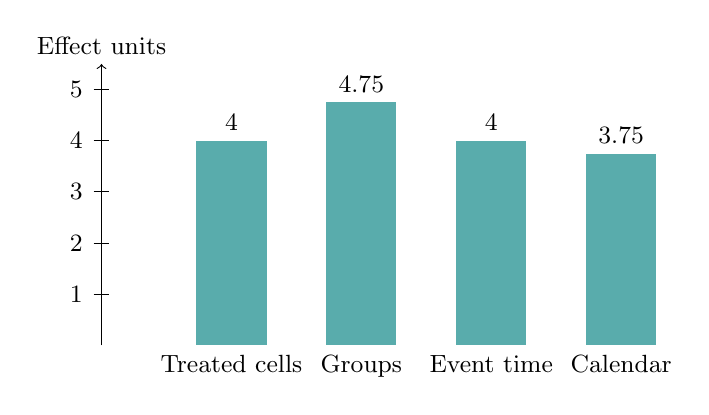
\begin{tikzpicture}[x=1.65cm,y=.65cm,every node/.style={font=\small}]
 \draw[->] (0,0)--(0,5.5) node[above]{Effect units};
 \foreach \y in {1,2,3,4,5}{\draw (-.06,\y)--(.06,\y);\node[left] at (-.07,\y){\y};}
 \foreach \x/\h in {1/4,2/4.75,3/4,4/3.75}{
  \fill[teal!65] (\x-.27,0) rectangle (\x+.27,\h);
  \node[above] at (\x,\h){\h};}
 \node[below,align=center] at (1,0){Treated\ cells};
 \node[below] at (2,0){Groups};\node[below] at (3,0){Event time};
 \node[below] at (4,0){Calendar};
\end{tikzpicture}
\caption{Different questions give different averages from the same constructed
panel. Values reproduce the two-cohort example in the R panel comparison.
They are defined averages, not empirical estimates or a ranking of packages.
\citep{exec24_panelr_contract}}
\label{reading:panel-averages}
\end{figure}

\subsection{When an implementation detail is consequential}
The selected routes in Section~\ref{rewrite:software-selection} use existing
procedures under declared targets and observation laws. A native port incurs
another implementation and validation burden; its benefit must cover that
burden. The inspected integration design develops that cost comparison.
\citep{exec16_s10_design}

These are proposal recommendations drawn from the preceding comparisons, not
claims that every integration has been executed. They also explain which
software details merit further investigation. A difference in coefficient
ordering is material when it changes reported uncertainty. A difference in a
random-number helper deserves priority only if it could change the statistical
conclusion or adoption choice. The conditional examples establish possible
failure mechanisms; they do not establish default-package defects or measured
coverage failures.~\citep{exec29_panel_inference_sources,exec29_panel_runtime_reference}

The longitudinal comparisons identify a more specific reason to withhold
some profiles. In the selected pygformula restriction path, deterministic
histories enter the fitting population even though simulation subsequently
enforces their known values. In the selected lmtp uncertainty composition,
the order of centering, weighting and aggregation matters when weights or
cluster sizes differ. The Julia survival comparison similarly separates
identified parameter combinations, observation entry and extrapolated tails.
These findings concern which distribution or uncertainty is computed, not
merely programming style. They narrow the proposed reuse contracts without
establishing how often failures occur in bank data.
Sections~\ref{sec:exec24-longitudinal-python}, \ref{rel23:ife-centering} and
\ref{rel22:survival-delegates} develop their source traces, exact constructions
and alternatives.~\citep{rel25pygfit,rel23ife,rel23ifecaller,rel22survbase,rel22survdist,rel22survcaller}

A source-level discrepancy can justify withholding an affected profile before
an empirical trial. It does not justify rejecting every method in the same
library, nor does a corrected formula alone establish native qualification.
The next comparison must reproduce the intended fitting population, output
scale and sampling unit, including adverse cases that expose those differences.
That requirement makes conditional reuse more precise: retain a useful original
method where its contract holds, repair and verify a specific mismatch, or
choose a substantively matched alternative.

The remaining uncertainty is specific to a candidate: its supported target,
version, reuse terms or performance on the proposed study. The commercial
comparison in Section~\ref{gap29:software-followup} distinguishes those
questions from missing bank entitlements and actual prices. An unobserved
capability remains unknown. The investment decision in
Chapter~\ref{rewrite:investment-decision} compares the resulting routes.


% SOURCE docs/release/2026-10-29/source/docs/writing-repair/2026-10-29/src/66540a8f29f1b949.tex CHAR 22969


\section{What the commercial comparison changes}
Commercial statistical packages are credible alternatives, not an empty space
waiting for the proposed service. The inspected Stata procedures cover distinct
treatment, panel, survival and structural questions; the SAS sources distinguish
statistical procedures from service access. The bank may already possess
trained staff and relevant entitlements. A proposal that ignores those assets
overstates the saving from a new platform.
\citep{exec13_ci_stata_causal_intro,exec18_gp_stata_xthdid,
exec14_survival_stata,exec13_ivrd_sas,exec23_workflow_sasctl}

Compare three feasible alternatives: improve existing analytical practice;
connect a small set of existing procedures; or build a broader common service.
For each study, distinguish a vendor-authored procedure, a community extension
inside a commercial host, an open client to a licensed server, and a general
numerical component. They have different support and cost implications. The
comparison has not established exact current prices, complete entitlements,
performance at the bank's scale or the absence of equivalent features in all
competitors. Those are unresolved commercial questions, not findings of
technical superiority.

The proposed investment is therefore conditional. Its candidate contribution
is a disciplined connection between the business question, assumptions,
software choices and financial interpretation. Fund a narrow comparison that
can show whether that connection prevents material errors or saves analyst
time. If the existing estate achieves the same result more cheaply, retain it.
If differences in estimands, graph interpretation or information dates repeatedly
change decisions, a shared service becomes more persuasive.



% SOURCE docs/release/2026-10-29/source/docs/writing-repair/2026-10-29/src/72f64a0c152b5f00.tex CHAR 0
\section{Existing commercial capabilities and their terms}
\label{gap29:software-followup}
The public experiment in Chapter~\ref{gap29:public} demonstrates why reuse is the starting point. Native
R fitting and a separate Python calculation agree on the same observations,
regression specification and HC2 covariance. Rewriting a familiar estimator
in another language would add little to that calculation. The proposal's
contribution must instead be demonstrated in the connection between the
economic question, assumptions, available information and reported decision.

\subsection{Panel estimation is already a commercial capability}
The official MATLAB documentation retrieved on 29 October 2026 describes
one-way fixed- and random-effects panel regressions. The fixed-effects
documentation explains transformed-data estimation, a subject-clustered
sandwich option and handling of missing measurements. It documents
\texttt{fitfepanel} as introduced in R2026b and
\texttt{fitrepanel} in R2026a. The retrieved pages are current R2026b pages;
their exact availability before the 7 October literature cutoff has not been
established. They are a dated capability update, not a reconstructed
pre-cutoff software comparison. \citep{gap29matlab}

The documented treatment of missing identifiers is consequential: a record
with an absent subject identifier is assigned an additional group, while a
missing predictor or response removes the observation from estimation.
Those are computational conventions, not evidence that the economic unit
is known or that discarded observations are ignorable. The panel study in
Chapter~\ref{gap29:funding} shows why that distinction matters.

A matched comparison must specify the institution and time effects,
covariance convention, initial sample and missing-record treatment before
comparing coefficients. The inspected pages describe a one-way model and
subject clustering; they are not sufficient evidence about every possible
way to obtain time effects or two-way covariance in the wider MATLAB estate.
There has been no licensed MATLAB execution in this study. The appropriate
proposal decision is to retain it as an existing-estate alternative and
test the declared calculation where the institution already has access.
Claims of missing commercial capability would require broader evidence.

\subsection{A decision diagram already contains an information structure}
HUGIN's official GUI 9.8 manual describes Bayesian networks, decision and
utility nodes, and limited-memory influence diagrams. Its account makes
the information available at each decision explicit through incoming
informational links; it also relaxes the traditional requirement that every
earlier observation remains available. This is directly relevant to a
servicing policy, where later actions must use the information actually
observed at their dates. \citep{gap29hugin}

The proposal should therefore compare a graph assistant with an established
diagram editor and a declared decision model. It should not equate drawing
an arrow with identifying an intervention effect, or infer from a manual
that the proposed integration has been implemented. The inspected material
supports a concrete alternative for representing decisions and information;
it does not establish an automatic solution to latent confounding or missing
outcomes.

The selected influence-diagram route has a further restriction that matters
for a loan portfolio: its manual excludes continuous chance nodes. The
separate conditional-Gaussian Bayesian-network facility does not remove
that restriction. That facility describes Gaussian variables whose means
are linear in their continuous parents, allows the coefficients and variances
to depend on discrete parents, and excludes continuous parents of discrete
nodes. These are different documented model families within the same
product. A continuous balance history therefore cannot be carried into the
decision diagram merely because another HUGIN model accepts a continuous
measurement. \citep{gap29hugin}

One possible comparator uses explicit balance and arrears categories in a
supplied decision model. Their boundaries, transition probabilities and
utilities would then be part of the economic approximation: customers in a
single category need not have the same response to a contact. A second
comparator retains continuous states in a separately justified policy-value
calculation, such as the construction in Chapter~\ref{rewrite:servicing} and
its fitted extensions. The choice should turn on whether categorisation
preserves the decision and its material uncertainty. The inspected manual
establishes the representation boundary; it does not quantify the loss from
coarsening a bank's records or demonstrate a native servicing trial.

The vendor's published licence text makes distribution using its API subject
to an OEM licence. That term changes the proposed reuse route: an internal
connection to an entitled installation and redistribution of a new product
are different propositions. The actual order, deployment conditions and
prices remain to be established with the vendor. The current manual's exact
release date relative to the literature cutoff is also unresolved.
\citep{gap29huginlicense}

\subsection{Which comparisons belong before a prototype}
The proposal can justify selecting existing estimators and diagram tools
from inspected methods, alternatives and explicit limitations. A complete
installed distribution, matched adverse-data tests and target-system
acceptance are subsequent implementation evidence. They must be specified
before a native adapter is accepted, but they should not be treated as
proof that the economic case for a prototype is unfinished in every respect.

The useful comparison asks whether an existing procedure answers the bank's
question and what additional work preserves its assumptions. Three choices
illustrate why conditional reuse can be justified before a new product is
built, while the meaning of a reported effect must be settled immediately.

\subsection{Reuse the estimator after choosing the population}
For an offer made once to each customer, the relevant average may cover all
eligible customers or only those who actually received the offer. DoubleML's
inspected Python interactive-regression implementation distinguishes these
targets, checks for a single binary treatment, and directs instrumental-variable
data to a different model. It forms separate predictions under treatment and
control, processes the propensity estimates, and constructs the corresponding
score. These are useful reasons to integrate the selected original procedure
instead of writing another implementation merely to change language.
The inspected revision is 6884b5f, dated 23 September 2026; its declared
BSD-3-Clause licence and dependencies are recorded separately from the earlier
installed-version observation. \citep{exec23_doubleml_reuse_source}

The recommendation is conditional integration of a specified model, with an
unadjusted or transparent adjusted comparison retained. Neither the choice of
predictor nor clipping a propensity establishes that every customer had a
realistic chance of receiving each action. Sampling dependence, permissible
covariates, target weights and the uncertainty calculation must agree with the
study. The full distribution and matched adverse-data trials belong in the
prototype comparison. Porting is justified only if a measured platform or
cost constraint outweighs the burden of maintaining the statistical procedure.

For phased adoption across branches, \texttt{did} offers a different target:
effects for an adoption cohort at a particular date, followed by an explicitly
chosen aggregation. The newly retrieved DESCRIPTION comes from the same
74b88eb commit as the retained API source. It identifies version 2.5.1.902,
R at least 4.1.0, a GPL-3 declaration and dependencies including DRDID.
Its bytes match the earlier mutable description, closing that specific
identity uncertainty. This is a repository version, not evidence of a stable
published release or of a complete deployment entitlement. A request for a
separate LICENSE file returned 404; that does not cancel the declaration.
\citep{survey29did,exec24_panelr_did}

The source's treatment of time-varying weights matters economically. In a
balanced panel the default comparison uses the earlier period's weights;
choosing varying weights switches to the repeated-cross-section estimator.
In an unbalanced panel, fixing weights at an anchor date restricts the sample
to units observed then. Thus two analysts can agree on the branch records yet
answer different questions after selecting different weighting rules. Imagine
two equally weighted customer groups with hypothetical effects of 10 and
$-10$ units. Their equally weighted effect is zero. If the analysis gives
the first group weight three and the second weight one, the weighted effect
is $(3\times10-10)/4=5$. This is a constructed arithmetic example, not a
\texttt{did} run: changing weights alone changes the population conclusion.
\citep{survey29didapi}

The appropriate proposal choice is an original R procedure with explicit
cohort, calendar, weighting and confidence-band definitions. A Python or
commercial comparison is useful when it implements the same target. The
selected API also distinguishes point estimates alone from influence-function
output required for inference and aggregation. Saving computation by requesting
only coefficients would therefore remove information needed for the proposed
investment decision. \citep{survey29didapi}

\subsection{Identification and numerical estimation do different jobs}
The inspected \texttt{causaleffect} documentation describes a symbolic answer
for an intervention distribution, optionally conditional on specified variables.
It returns a formula or structured probability expression when the query is
identified under the supplied graph; a nonidentification path reports the
graphical obstruction. The graph convention represents hidden common causes
through specially marked edges. Its selected source is version 1.3.17 at
ff6059f; the package Date field and commit timestamp disagree, so that
revision is described by its exact saved identity. \citep{exec18_rid_causaleffect}

This supports a bounded role as an identification reference alongside the
chosen graph representation. It does not choose the bank's causal graph,
estimate the formula from customer records, or produce a sampling interval.
Those tasks need separate evidence. Before accepting an implementation, compare
an adjustment case, a genuinely nonidentified case and a conditional query;
preserve variable names, hidden-edge marks and the distinction between an
unidentified effect and a computation that failed. Ananke or aGrUM can remain
alternatives where their documented query and hidden-variable semantics match.
There is no scientific reason to port the symbolic algorithm until a concrete
constraint makes the original implementation unsuitable.

\subsection{Compare with a named commercial service}
The current causaLens pages identify a specific service to compare: Digital
Workers assembled through the Digital Worker Factory, with the System of Work
for management and monitoring. The pages describe portable containers,
connections to existing business systems, human review and escalation, and
advertise human-guided causal discovery, causal model building, root-cause
analysis and intervention optimisation. These observations were made on
29 October 2026; no pre-cutoff availability or equivalence to an earlier
DecisionOS offering is inferred. \citep{survey29causalens}

This changes the commercial comparison. A proposal based only on graph editing,
ordinary system connections or automated reports cannot treat those functions
as unserved demand. The useful question is whether the proposed combination
improves the formulation of an economic choice, the treatment of identifying
assumptions, uncertainty and the analyst's time at a competitive total cost.
The vendor's pages establish advertised scope. They do not expose, in the
inspected material, a versioned causal-estimation specification, an independently
reconstructable comparison, a price or the bank's contractual rights.
Consequently their performance multipliers and return claims are not used as
measured advantages in this proposal. \citep{survey29causalens}

A fair later comparison would give both approaches the same information about
an offer or servicing decision, including a case with an omitted cause and a
case with outcome-dependent loss of records. It would evaluate the target
chosen, assumptions stated, consequential errors, uncertainty, time and full
cost. Correctly requesting missing information can be a better answer than a
confident numerical recommendation. The current source evidence supports
including the named commercial service in that comparison; actual superiority,
licensing and adoption remain to be established.


% SOURCE docs/release/2026-10-29/source/docs/writing-repair/2026-10-29/src/626099247fe4b6ef.tex CHAR 0
\section{The selected routes and the comparisons that could change them}
\label{rewrite:software-selection}

The preceding seventeen-area synthesis explains the methods and their
restrictions. The selection here turns that analysis into an order of work.
The immediate offer study uses the transparent cell-mean estimator already
demonstrated. More flexible effects, discovered diagrams and dynamic policies
enter only when the question requires them. A source-supported candidate is
selected for a bounded comparison; it is not declared a winner on speed,
coverage or institutional cost before that comparison is performed.

\subsection{The initial route and its serious alternatives}
For the first offer question, retain the saturated cell means as the
independently understandable comparator. If adjustment must extend beyond
these two strata, compare an explicitly population-targeted effect procedure
with the relevant EconML specification, rather than accepting the default
constant projection as the requested average. The inspected EconML revision
declares 0.17.0; its commit is dated 1 October 2026. R grf and documented
Stata effect procedures are serious alternatives when their target and
uncertainty match the study. The current environment's absence of a package
is an execution constraint, not evidence that the method is inferior.
\citep{exec19_econml_source,exec13_grf_rpath,exec13_ch_stata}

If a supplied diagram is disputed, use the inspected causal-learn 0.1.4.8
as the first Python discovery candidate and pcalg 2.7-12 as the R comparator
for the same restricted PC or FCI question. This is a composition choice
for a Python-facing prototype, not a ranking of discovery algorithms.
Match the test, search options, hidden-cause assumptions and returned graph
class. Java Tetrad remains a genuine alternative where its model and tests
fit better. Do not replace several causal explanations with one arrow
orientation to simplify the interface.
\citep{v12_sw_causallearn,exec13_pcalg_reuse_primary,exec13_java_tetrad}

For symbolic identification of a supplied admissible graph, the selected
Ananke 0.5.0 source supplies a Python candidate and aGrUM/pyAgrum supplies
a distinct comparator. Keep a query's identified expression separate from
a model-oracle numerical answer. For longitudinal extension, compare the
inspected gfoRmula revision, which declares 1.1.2 with release date still
TBD, with pygformula 1.2.1. The former declaration is not treated as proof
of a released 1.1.2 binary. The complete history, event order, interventions
and resampling procedure must be matched before drawing a reuse conclusion.
For the selected pygformula revision, withhold the documented deterministic
covariate-restriction profile until its fitting-population mismatch is corrected
and verified. This restricts that profile rather than treating every simulator
output as invalid (Section~\ref{sec:exec24-longitudinal-python}).
\citep{exec24_ananke_source,exec19_cxx_identification_source,
exec24_agrum_source,exec20_gformula_reuse,exec24_longpy_pygformula_source}

\subsection{Disposition across the required causal areas}
The matrix specifies the first candidate or the reason a unique choice
would be premature. The cited editions are the retained cutoff sources,
not a search for the newest releases. Every row is an authored integration
recommendation based on the preceding source comparison. No new package
benchmark was executed for this matrix.

\begingroup\small
\begin{longtable}{P{2.2cm}P{4.3cm}P{7.7cm}}
\toprule Area & Candidate and serious alternative & Restriction and observation that changes the choice\\\midrule
\endfirsthead
\toprule Area & Candidate and serious alternative & Restriction and observation that changes the choice\\\midrule
\endhead
1. Independent discovery & causal-learn PC; pcalg or Tetrad comparator & Begin with a matched independent-observation test and graph class. Mixed measurements or unsupported tests can favour the alternative. Retain unresolved directions. \citep{v12_sw_causallearn,exec13_pcalg_reuse_primary,exec13_java_tetrad}\\[5pt]
2. Hidden causes & causal-learn FCI; pcalg latent route & Use the specified ancestral-graph interpretation. A need for a point effect that the class cannot identify requires new information, not a preferred orientation. \citep{v12_sw_causallearn,exec13_pcalg_reuse_primary}\\[5pt]
3. Temporal discovery & Tigramite; supplied structural time-series model & Keep calendar gaps, lag choices and graph ambiguity. A crisis regime or inadequate observation history can invalidate the candidate's stationary comparison. \citep{exec23_tigramite_reuse_source,exec13_ct_stata_svar}\\[5pt]
4. Identification & Ananke; aGrUM/pyAgrum & Match hidden-variable model and query semantics. Unsupported query classes or model-only numerical answers block an observational identification claim. \citep{exec24_ananke_source,exec24_agrum_source}\\[5pt]
5. Effects and heterogeneity & Transparent target-weighted means first; EconML, grf or Stata when needed & Additional adjustment or heterogeneity changes the method requirement. Match population weights and uncertainty; a constant projection is not automatically the population effect. \citep{exec19_econml_source,exec13_grf_rpath,exec13_ch_stata}\\[5pt]
6. IV and thresholds & Existing team's IV procedure; rdrobust for a justified threshold & No unique IV vendor is preferred without the team's design and entitlement. Weak instruments, bandwidth sensitivity or an unmatched complier population can defeat the proposed decision. \citep{exec13_ivrd_stata,exec13_ivrd_sas,exec13_ivrd_rdrobust}\\[5pt]
7. Longitudinal effects & gfoRmula; pygformula comparator & Begin with a short fixed policy and observed histories. Compare entire simulation and uncertainty routes; withhold the selected pygformula covariate-restriction profile pending correction and verification. Missing action determinants or sparse histories require a new design. \citep{exec20_gformula_reuse,exec24_longpy_pygformula_source,rel25pygfit}\\[5pt]
8. Policy learning & Fixed rule first; policytree for a supported static extension & Separate action-score construction, optimization and evaluation. Dynamic regimes require dtrreg/polle-type histories rather than relabelling a static tree. \citep{exec24_policiesr_policytree,exec24_policiesr_dtrreg,exec24_policiesr_polle}\\[5pt]
9. Panel adoption & R did group-time route; Python differences and Stata comparator & Choose aggregation before software. The inspected did declaration is 2.5.1.902, not a claim of a released stable version. Missing cohorts or calendar dependence can change scope and uncertainty. \citep{exec24_panelr_did,exec24_panelpy_differences,exec18_gp_stata_xthdid}\\[5pt]
10. Synthetic controls & Synth route; CausalImpact as a different model comparison & Neither universally dominates. Donor eligibility, pre-period fit and stability determine the useful comparison. A community extension in Stata is not vendor-authored merely because the host is commercial. \citep{exec19_synth_stata_source,exec13_ci_r,exec13_ci_semantics}\\[5pt]
11. Dynamic funding & Stata/EViews documented design-specific routes; no universal choice & Instruments, shock restrictions and effective calendar must be fixed first. A generic lagged regression cannot choose the bank's structural shock or validate its inference. \citep{exec19_dynamic_stata_ab,exec19_dynamic_stata_system,exec19_dynamic_stata_lp,exec19_dynamic_eviews_panel}\\[5pt]
12. Spillovers & MossSpider for its network construction; inferference for grouped allocation & These are distinct exposure and assignment models. Obtain the economically relevant links and mechanism before selecting between them. \citep{exec24_interference_mossspider,exec24_interference_inferference}\\[5pt]
13. Mediation & R mediation; documented Stata procedure & Choose the mechanism intervention and sensitivity range. Randomized treatment alone does not establish the extra mediation restrictions. \citep{exec24_mediation_original,exec24_mediation_sources,exec13_ci_stata_mediate}\\[5pt]
14. Transfer and missingness & Explicit target weighting plus justified imputation; existing Stata/SAS facilities & A single package choice remains unresolved until the selection and missingness law is specified. Existing commercial imputation can be sufficient; it does not identify unrestricted transport. \citep{pearltransport2014,exec21_transport_stata_mi,exec21_transport_sas_mi_intro}\\[5pt]
15. Hidden-state inference & PyMC or Stan for a supplied model; commercial state-space route & Prefer the engine already supporting the model. Development sources are not release or convergence evidence. Model meaning, prior sensitivity and diagnostics decide reuse. \citep{exec23_pymc_sources,exec25_bsw_stan,exec22_state_stata_sspace_post}\\[5pt]
16. Observation construction & DuckDB for the initial analysis view; Polars or existing warehouse & DuckDB v1.4.0 is the inspected baseline. Reuse an existing view if equivalent; add historical feature tooling only when availability and revisions demand it. Truthful links and dates remain substantive inputs. \citep{exec19_duckdb_source,exec23_polars_sources,exec19_feast_source}\\[5pt]
17. Computation and delivery & Reuse complete procedures; retain numerical kernels as components & Compare full sample, covariance and reporting behavior across library/CLI/MCP. Port only for a demonstrated constraint; agreement of bridges to one engine is not independent corroboration. \citep{exec25_paneljava_commons,exec25_panelcxx_fixest,exec25_panelother_julia}\\
\bottomrule
\end{longtable}
\endgroup

A missing comparison matters when it can change one of these choices. The
first practical uncertainties are the available pinned execution environment,
the equivalence of the selected procedure's target and uncertainty, and
whether a present commercial entitlement supplies the same complete output
more cheaply. Completing every language--area cell is not a prerequisite
for this bounded prototype, but it remains an open survey obligation if a
broader comparative claim is made. The source register retains exact commits,
versions, technical anchors and known omissions for each cited candidate.


% SOURCE docs/release/2026-10-29/source/docs/writing-repair/2026-10-29/src/66540a8f29f1b949.tex CHAR 24851


\section{What remains to be learned}
The seventeen areas now lead to explicit provisional choices, but this synthesis
does not complete the underlying census. There is no claim that every
language--area pair has been exhaustively searched or that every candidate has
been executed. Complete dated source and capability comparisons where a missing
candidate could change the preferred route. Compare actual implementations on
matched questions before claiming numerical agreement. Obtain edition,
entitlement and price information before a purchase recommendation. Investigate
transitive numerical details only where they could change the inference or
the selected integration.

Some limits require new information rather than more programming: unidentified
effects under unrestricted confounding, absent support for a proposed action,
unknown assignment histories and uncertain transfer to a new population. State
the restrictions or data that would narrow each limit. These findings can
support a useful proposal even when they do not support a universal product.


